\begin{frame}{第二十七讲、反常积分}
	\linespread{1.5}
	\begin{enumerate}
	  \item {\bf 内容与要求}{\b( \S 6.5 )}
	  \begin{itemize}
	    \item 理解反常积分的概念
	    \item 掌握基本的反常积分判定方法
	  \vspace{1em}
	  \end{itemize}
	  \item {\bf 课后作业:}
	  \begin{itemize}
 	    \item 书面作业:
	     {\b 习题6.5:1(4-6),2(1,4,6),5,8}
% 	    \item {\b 习题6.3:8,9,12,14,18}
%   	    \item 思考题:{\b 习题6.4:1-30其余各题}
	  \end{itemize}
	\end{enumerate}
\end{frame}

\begin{frame}{定积分存在的条件}
	\linespread{1.5}
	$$\alert{I=\dint_a^bf(x)\d x}$$
	\begin{enumerate}\pause 
	  \item {\bf 有限区间:}$a,b\ne \infty$\pause 
% 	  \begin{itemize}
% 	    \item 
% 	  \end{itemize}
	  \item {\bf 分段连续:}$f(x)$最多有限多个第一类间断点\pause 
% 	  \begin{itemize}
	    \item {\bf 必要条件:}$f(x)$有界
% 	  \end{itemize}
	\end{enumerate}
\end{frame}

\section{无穷限的反常积分}

\begin{frame}{无穷限的反常积分}
	\linespread{1.2}\pause 
	\begin{block}{{\bf 定义6.5.1:}(无穷积分)\hfill P380}
		$$\alert{\dint_a^{+\infty}f(x)\d x}\pause
		=\lim\limits_{t\to+\infty}\dint_a^tf(x)\d x$$ \end{block}\pause 
	\begin{itemize}
	  \item 类似地,可以定义$\alert{\dint_{-\infty}^af(x)\d x}$和
		$\alert{\dint_{-\infty}^{+\infty}f(x)\d x}$\pause 
	  \item Newton-Leibnitz公式\pause 
	  $$\dint_a^{+\infty}f(x)\d x=F(x)|_{a}^{+\infty}
	  =\limx{+\infty}F(x)-F(a)$$
	\end{itemize}
\end{frame}

\begin{frame}
	\linespread{1.2}
	\begin{exampleblock}{{\bf 例1:}计算以下无穷限积分\hfill P381:例1}
		\begin{enumerate}
		  \item $\dint_{-\infty}^{+\infty}\df{1}{1+x^2}\d x$
% 		  \item $\dint_0^{+\infty}te^{-pt}dt,\;p>0$
% 		  \item $\dint_a^{+\infty}\df{\d x}{x^p},\;p>0$
		\end{enumerate}
	\end{exampleblock}\pause 
	\begin{center}
			\resizebox{!}{5cm}{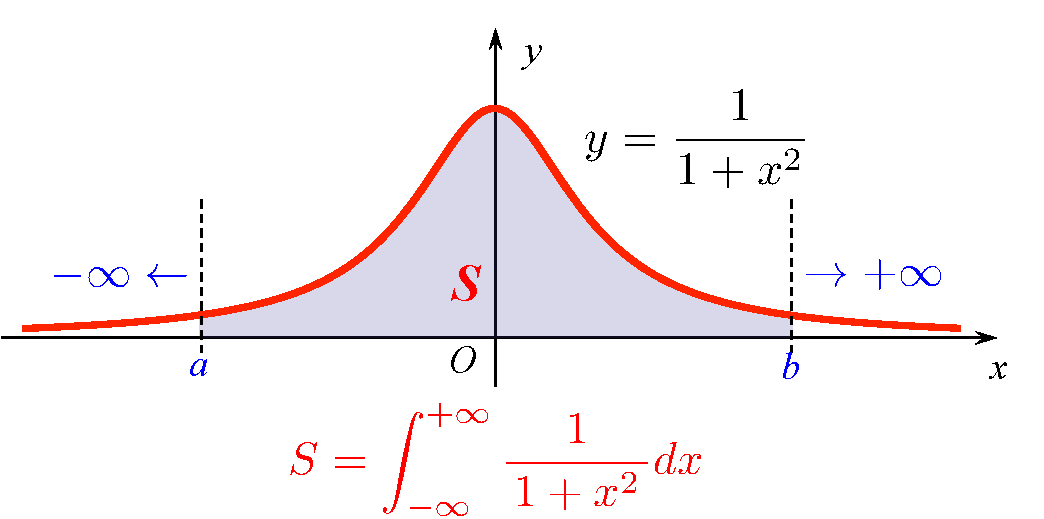
\includegraphics{./images/ch6/infint.pdf}}
		\end{center}
\end{frame}

\begin{frame}
	\linespread{1.2}
	\begin{exampleblock}{{\bf 例2}\hfill P382-例3,P384-例5}\pause 
		\begin{enumerate}
		  \item 讨论$\dint_a^{+\infty}\df{\d x}{x^p},\;a>0, p>0$的敛散性;\pause 
		  \item 证明$$\dint_1^{n+1}\df 1{x^p}\d x<\sum\limits_{k=1}^n\df 1{k^p}
		  <1+\dint_1^n\df{1}{x^p}\d x$$\pause 
		  \item 根据以上结论给出$p$级数的判敛条件。
		\end{enumerate}
	\end{exampleblock}
\end{frame}

\section{无界函数的反常积分}

\begin{frame}{无界函数的反常积分}
	\linespread{1.2}\pause 
	\begin{block}{{\bf 定义6.5.2}\hfill P385}
		\begin{enumerate}\pause 
		  \item {\bb 瑕点:}无穷间断点\pause 
		  \item 设$a$为$f(x)$的瑕点,{\bb 瑕积分:}
		  $$\dint_a^bf(x)\d x=\limx{a^+}\dint_t^bf(x)\d x$$
		\end{enumerate}
	\end{block}\pause 
	\begin{exampleblock}{{\bf 例3}\hfill P386-例6}
		计算瑕积分$\dint_0^a\df{1}{\sqrt{a^2-x^2}}\d x,\;a>0$。
	\end{exampleblock}
\end{frame}

\begin{frame}
	\linespread{1.2}
	\begin{exampleblock}{{\bf 例4:}讨论瑕积分的收敛性\hfill P387-例7}
		\begin{columns}\pause 
			\column{0.5\textwidth}
				\begin{enumerate}
				  \item $\dint_{-1}^1\df{\d x}{x^2}$\pause 
				\end{enumerate}
			\column{0.5\textwidth}
				\begin{enumerate}
				  \addtocounter{enumi}{1}
				  \item $\dint_{-1}^1\df{\d x}{x}$
				\end{enumerate}
		\end{columns}
	\end{exampleblock}\pause 
	\bigskip
	\begin{exampleblock}{{\bf 例5:}\hfill}
		计算积分:$$\dint_0^{+\infty}\df{\d x}{\sqrt{x(x+1)^3}}$$
	\end{exampleblock}
\end{frame}

\section{反常积分收敛性的判定}

\begin{frame}{反常积分收敛性的判定}
	\linespread{1.2}\pause 
	{\bf 注:}以下讨论均以无穷积分为例\pause 
	\begin{block}{{\bf 定理6.5.3:}(比较判别法)\hfill P389}\pause 
		设$f(x),g(x)$在$[a,+\infty)$上连续,且
		$$0\leq f(x)\leq g(x),\quad x\in[a,+\infty)$$\pause 
		\vspace{-1em}
		\begin{enumerate}
		  \item
		  $\dint_a^{+\infty}g(x)\d x$收敛$\Rightarrow\dint_a^{+\infty}f(x)\d x$收敛\pause 
		  \item $\dint_a^{+\infty}f(x)\d x$发散$\Rightarrow\dint_a^{+\infty}g(x)\d x$发散
		\end{enumerate}
	\end{block}
\end{frame}

\begin{frame}
	\linespread{2}
	\begin{exampleblock}{{\bf 例5:}讨论以下无穷积分的敛散性\hfill P388-例1}
		\begin{enumerate}\pause 
		  \item $\dint_2^{+\infty}\df{1+\sin x}{x^2}\d x$\pause 
		  \item $\dint_1^{+\infty}\df{\d x}{\sqrt[3]{x^4+1}}$
		\end{enumerate}
	\end{exampleblock}
\end{frame}

\begin{frame}{比较判别法的极限形式}
	\linespread{1.2}\pause 
	\begin{alertblock}{{\bf 定理}(极限判别法)\hfill}
		设$f(x),g(x)$在$[a,+\infty)$上连续,
		$0\leq f(x)\leq g(x)$,且
		$$\limx{+\infty}\df{f(x)}{g(x)}=l$$\pause 
		\vspace{-1em}
		\begin{enumerate}
		  \item $0<l<+\infty$,两个无穷积分同敛散\pause 
		  \item
		  $l=0$,$\dint_a^{+\infty}g(x)\d x$收敛$\Rightarrow\dint_a^{+\infty}f(x)\d x$收敛\pause 
		  \item
		  $l=+\infty$,$\dint_a^{+\infty}f(x)\d x$发散$\Rightarrow\dint_a^{+\infty}g(x)\d x$发散
		\end{enumerate}
	\end{alertblock}
\end{frame}

\begin{frame}
	\linespread{1.2}
	\begin{exampleblock}{{\bf 例6:}判定以下反常积分的收敛性\hfill}
		\begin{enumerate}\pause 
		  \item $\dint_1^{+\infty}\df{\d x}{x\sqrt{1+x^2}}$\pause 
		  \item $\dint_1^{+\infty}\df{x^{3/2}}{1+x^2}\d x$\pause 
		  \item $\dint_1^{+\infty}\df{\arctan x}{x}\d x$
		\end{enumerate}
	\end{exampleblock}
\end{frame}

\begin{frame}{绝对收敛性}
	\linespread{1.2}\pause 
	\begin{alertblock}{{\bf 定理}(绝对收敛性)\hfill}
		设$f(x)$在$[a,+\infty)$上连续,若$\dint_a^{+\infty}|f(x)|\d x$收敛,则
		$\dint_a^{+\infty}f(x)\d x$收敛。
	\end{alertblock}\pause 
	\begin{exampleblock}{{\bf 例7}\hfill}
		讨论反常积分$\dint_0^{+\infty}e^{-ax}\sin bx\d x\;(a>0)$的敛散性。
	\end{exampleblock}
\end{frame}

\begin{frame}{瑕积分的敛散性}
	\linespread{1.2}\pause 
	\begin{exampleblock}{{\bf 例8:}判定下列积分的敛散性\hfill}\pause 
		\begin{enumerate}
		  \item $\dint_1^3\df{\d x}{\ln x}$\pause 
		  \item $\dint_0^1\df{\d x}{\sqrt{(1-x^2)(1-k^2x^2)}}\;(k^2<1)$\pause 
		  \item $\dint_0^1\df 1{\sqrt{x}}\sin\df 1x\d x$
		\end{enumerate}
	\end{exampleblock}
\end{frame}

\section{$\Gamma$函数}

\begin{frame}{$\Gamma$函数}
	\linespread{1.2}
	$$\alert{\Gamma(s)=\dint_0^{+\infty}e^{-x}x^{s-1}\d x\;(s>0)}$$\pause 
	\begin{alertblock}{{\bf 常见性质}\hfill}\pause 
		\begin{enumerate}
		  \item $\Gamma(s+1)=s\Gamma(s)$\pause 
		  \item $\lim\limits_{s\to 0+}\Gamma(s)= +\infty$\pause 
		  \item $\Gamma(s)\Gamma(1-s)=\df{\pi}{\sin \pi s}\;(0<s<1)$\pause 
		  \item $2\dint_0^{+\infty}e^{-x^2}\d x=\Gamma\left(\df 12\right)=\sqrt{\pi}$
		\end{enumerate}
	\end{alertblock}
\end{frame}

\begin{frame}[<+->]{小结}
	\linespread{1.5}
	\begin{enumerate}
	  \item {\bf 反常积分的概念}
	  \begin{itemize}
	    \item 与无穷级数的类比
	    \item 两类反常积分的相互转换
	  \end{itemize}
	  \item {\bf 反常积分的收敛性判定}
	  \begin{itemize}
	    \item 比较法
	    \item 极限法
	    \item 绝对收敛性
	  \end{itemize}
	\end{enumerate}
\end{frame}

%====================================

% \begin{frame}{title}
% 	\linespread{1.2}
% 	\begin{block}{{\bf title}\hfill}
% 		123
% 	\end{block}
% \end{frame}